\documentclass[11pt, spanish]{article}
\usepackage[utf8]{inputenc}
\usepackage{listings} 
\usepackage{graphicx}
\usepackage{amsfonts}
\usepackage[dvipsnames]{xcolor}
\usepackage[T1]{fontenc}
\usepackage{bigfoot}
\usepackage{amsmath}
\usepackage[numbered,framed]{matlab-prettifier}
\usepackage{caption}
\usepackage[figurename=Figura, tablename=Tabla, font={small,tt}]{caption}
\usepackage{blkarray}
\usepackage{xcolor}
\usepackage{multicol}
\usepackage[]{algorithm2e}
\usepackage{float}
\usepackage[section]{placeins}

\makeatletter
    \setlength\@fptop{0\p@}
\makeatother

\date{}

\usepackage{geometry}
 \geometry{
 a4paper,
 left=30mm,
 right=30mm,
 top=30mm,
 }

\lstset{
	style              = Matlab-editor,
  	basicstyle         = \mlttfamily,
  	escapechar         = ",
  	mlshowsectionrules = true,
	framesep=4.5mm,
	framexleftmargin=2.5mm,
	fillcolor=\color{White},
	rulecolor=\color{Black},
	numberstyle=\normalfont\tiny\color{Black}
}

\captionsetup[lstlisting]{font={small,tt}}
\renewcommand{\lstlistingname}{Script}
\newcommand\RED{\color{red}}
\newcommand\BLUE{\color{blue}}
\newcommand{\BigO}[1]{\ensuremath{\operatorname{O}\bigl(#1\bigr)}}
\newcommand{\norm}[1]{\left\lVert#1\right\rVert}

\begin{document}

\renewcommand\lstlistlistingname{Lista de Scripts}

\author{Sebastián Valencia Calderón \\ 201111578}
\title{Laboratorio 7: Integración numérica en \textsc{Matlab}.}
\maketitle

%====================================================================
\section{Introducción}

Desde los cursos de cálculo elemental, se conoce el proceso analítico para hallar las integrales definidas y no definidas de una función analítica. Se conocen métodos analíticos para su solución y las aplicaciones de la integración. Sin embargo, en el desarrollo de las ciencias y de la ingeniería, resulta conveniente hallar métodos numéricos para la solución aproximada de integrales, haciendo uso de algoritmos numéricos. Un ejemplo típico de aplicación indirécta de estos métodos a problemas en ciencias e ingeniería, es la solución numérica o mixta de ecuaciones diferenciales ordinarias. (Referencias [3], [5]).\\

Existen varios métodos para la solución de este problema. Los más elementales son los del trapecio, y el basado en la regla de Simpson, el presente laboratorio, presenta la solución de algunos problemas para ser resueltos haciendo uso de integración numérica, para integración en $\mathbb{R}$, $\mathbb{R}^2$, y $\mathbb{R}^3$. El desarrollo de estos problemas, corresponde más a un estudio de los métodos dispuestos de manera nativa en \textsc{Matlab}, que un estudio del diseño y desarrollo de los mismos, por lo tanto, se pretende aprender a usar las funciones \texttt{trapz()}, \texttt{quad()}, \texttt{quad2d()}, y \texttt{triplequad()}. De manera concreta, el desarrollo de los ejercicios, pretende comprometerse con el siguiente objetivo:

\begin{enumerate}
\item Presentar y reconocer el funcionamiento de algunos algoritmos de integración numérica en \textsc{Matlab}.
\end{enumerate}

%==================================================================
\section{Procedimiento}

Para cumplir los objetivos enumerados anteriormente, se estudia el uso de los métodos básicos de integración numérica. Es decir, los enumerados en la introducción. Con estos, se desarrolla un script para comparar su desempeño sin tener en cuenta su implementación o diseño, sólo su uso, y a partir del uso de ellos en cuatro funciones se compra su desempeño y casos de uso en la práctica, además, se puede inferir sobre su diseño e implementación. Posteriormente, se estudia el uso de las funciones dispuestas en \textsc{Matlab}, para la integración en dimensiones mayores.\\

%==================================================================
\section{Resultados}

A continuación, se exponen los resultados  y las herramientas de ejecución para cada uno de los problemas propuestos.

\subsection{Método del trapecio y de Simpson en una dimensión en \textsc{Matlab}}

Haciendo uso de las funciones disponibles en \texttt{Matlab} para la integración numérica por los métodos del trapecio y de Simpson, se calculan las siguientes integrales en el intervalo $0 \leq x \leq 15$. Se explican y justifican los parámetros empleados para esto.\\

$$C(x) = \int_{0}^{x} \cos \left(\frac{\pi \tau^2}{2}\right)\ d \tau \quad S(x) = \int_{0}^{x} \sin \left(\frac{\pi \tau^2}{2}\right)\ d \tau \quad $$\
$$C_1(x) = \int_{0}^{x} \cos \left(\tau^2\right)\ d \tau \qquad S_1(x) = \int_{0}^{x} \sin \left(\tau^2\right)\ d \tau$$\

\lstinputlisting[caption = {Evaluación de las integrales enunciadas, en el intervalo $0 \leq x \leq 15$, haciendo uso de las dos funciones de \textsc{Matlab}. (\textbf{functions.m})}]{data/scripts/functions.m}\

El script anterior, muestra la evaluación iterativa para cada punto del vector de integración de cada una de las funciones, el uso de la función de \textsc{Matlab} para el método del trapecio (\texttt{trapz()}), requiere la función a integrar y un vector de la evaluación del vector de integración hasta el punto actual. Asimismo, la regla de Simpson, requiere la función, y ambos límites de integración. Esto es implementado haciendo uso de la función \texttt{quad()}. Los scripts para graficar, no se incluyen por su poca relevancia con el problema en cuestión.\\

El scrip referido, el cual contiene las definiciones de las funciones es:

\lstinputlisting[caption = {Definición de las funciones a integrar. (\textbf{definitions.m})}]{data/scripts/definitions.m}\

A continuación, se incluye la gráfica de la integral, obtenida a partir de los métodos numéricos referidos anteriormente. Esto para la primera función.

\begin{figure}[H]
\centering
	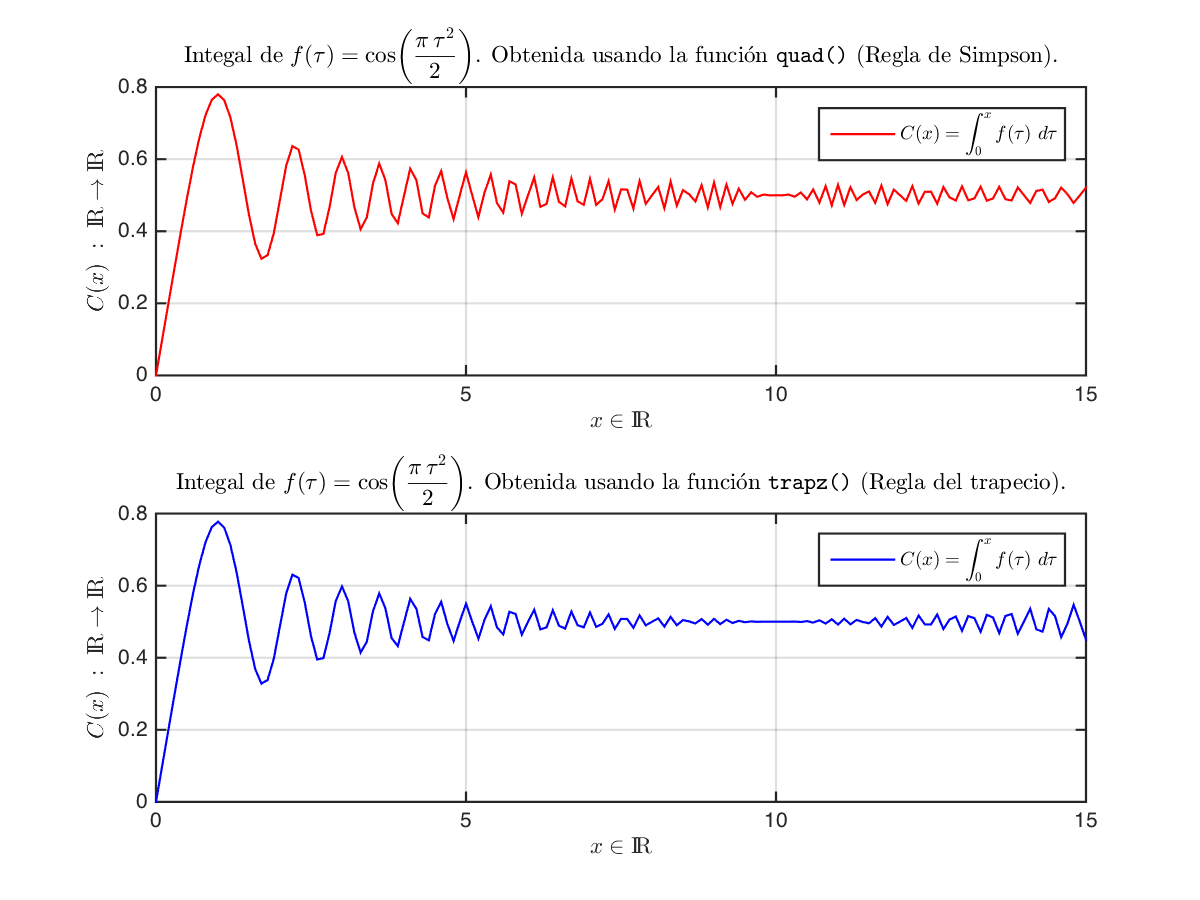
\includegraphics[scale=0.8]{data/img/f1intplot01}
	\caption{Integral de $f_1(x)$, obtenida numéricamente haciendo uso de las dos funciones referidas, para $0 \leq x \leq 15$, con pasos de 0.1.}
\end{figure}

Ahora, se incluyen las gráficas para las demás funciones.

\begin{figure}[H]
\centering
	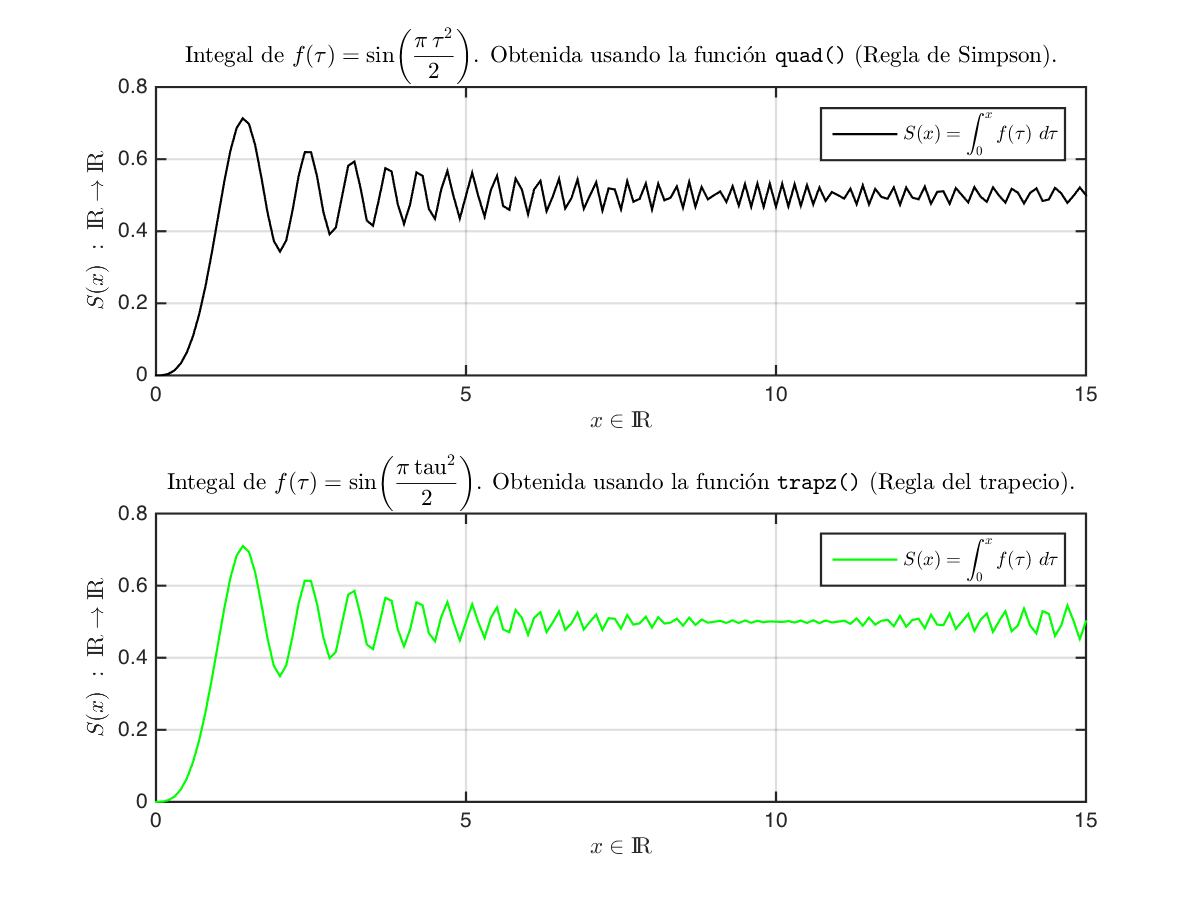
\includegraphics[scale=0.6]{data/img/f2intplot01}
	\caption{Integral de $f_2(x)$, obtenida numéricamente haciendo uso de las dos funciones referidas, para $0 \leq x \leq 15$, con pasos de 0.1.}
\end{figure}

\begin{figure}[H]
\centering
	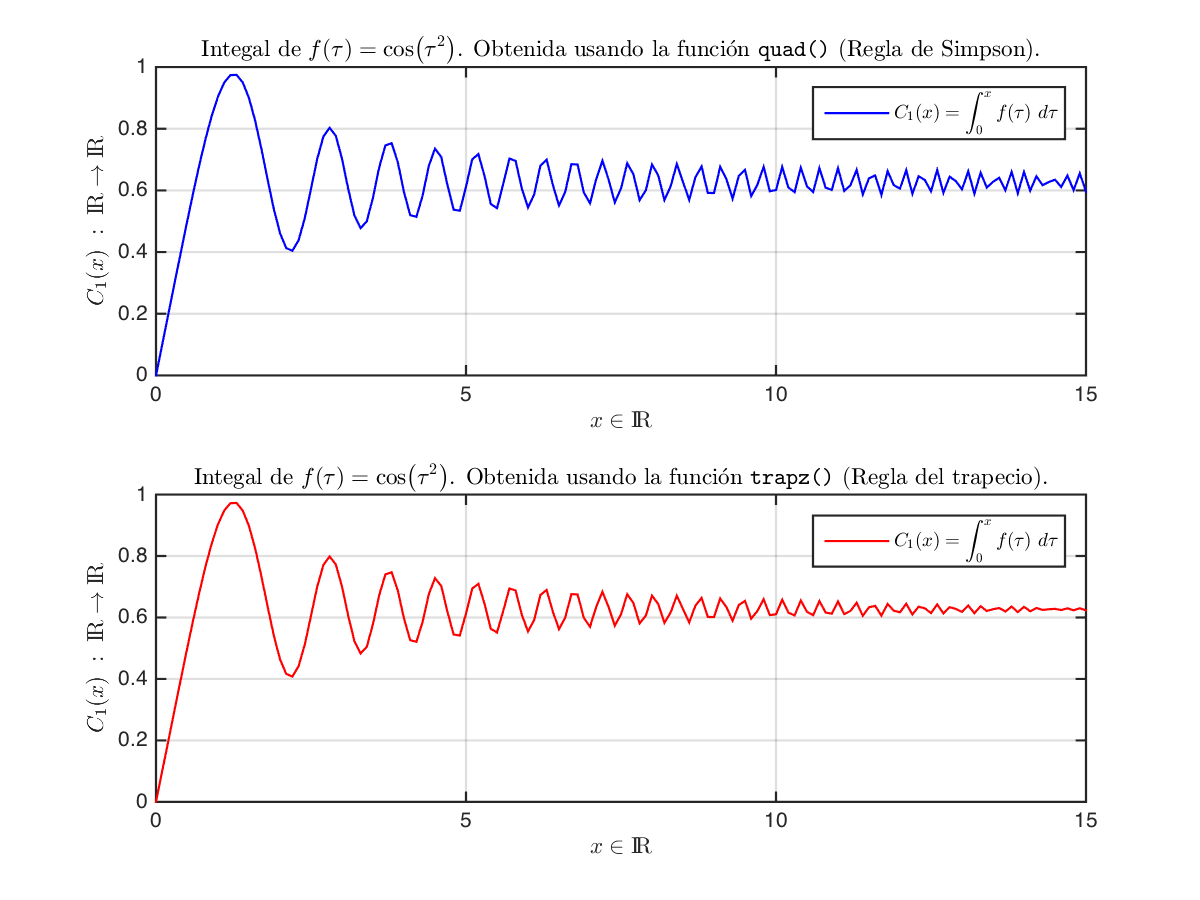
\includegraphics[scale=0.6]{data/img/f3intplot01}
	\caption{Integral de $f_3(x)$, obtenida numéricamente haciendo uso de las dos funciones referidas, para $0 \leq x \leq 15$, con pasos de 0.1.}
\end{figure}

\begin{figure}[H]
\centering
	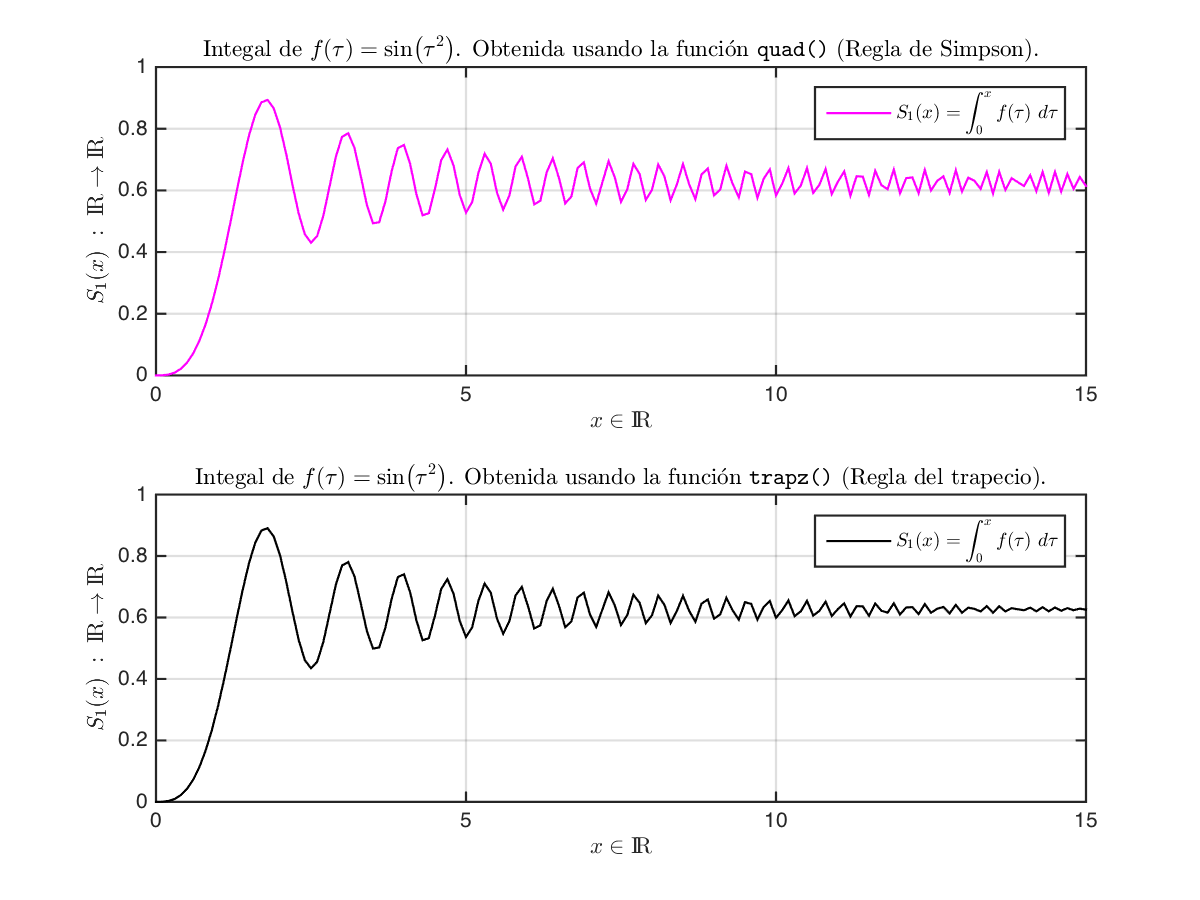
\includegraphics[scale=0.8]{data/img/f4intplot01}
	\caption{Integral de $f_4(x)$, obtenida numéricamente haciendo uso de las dos funciones referidas, para $0 \leq x \leq 15$, con pasos de 0.1.}
\end{figure}\

Haciendo uso de estas visualizaciones gráficas para cada una de las integrales con los dos métodos, es difícil inferir a cerca del desempeño de cada una en comparación con la otra. Es decir, con estas gráficas, no se observa a primera vista si una es mejor a la otra para el cálculo de la integral numérica de una función analítica. Para mitigar este problema, se hace más preciso el vector de integración, es decir, el paso se agudiza para tener mayores valores en el intervalo de integración, esto corresponde a cambiar el valor de \texttt{step} en el primer script (linea 2), a 0.001. El script, toma más tiempo en correr. \\

Las figuras de esta última simulación, se encuentran a continuación. En estas se observa una especie de ruido obtenido mediante el uso de la regla de Simpson, mientras que emplear la regla del trapecio, resulta en una curva mucho más suave y definida que la otra. Esto último, permite inferir que el desempeño en resultados de la regla del trapecio, haciendo la comparación mediante la forma de la función integral, es mucho mayor. Sin embargo, el resultado numérico es aproximado.

\begin{figure}[H]
\centering
	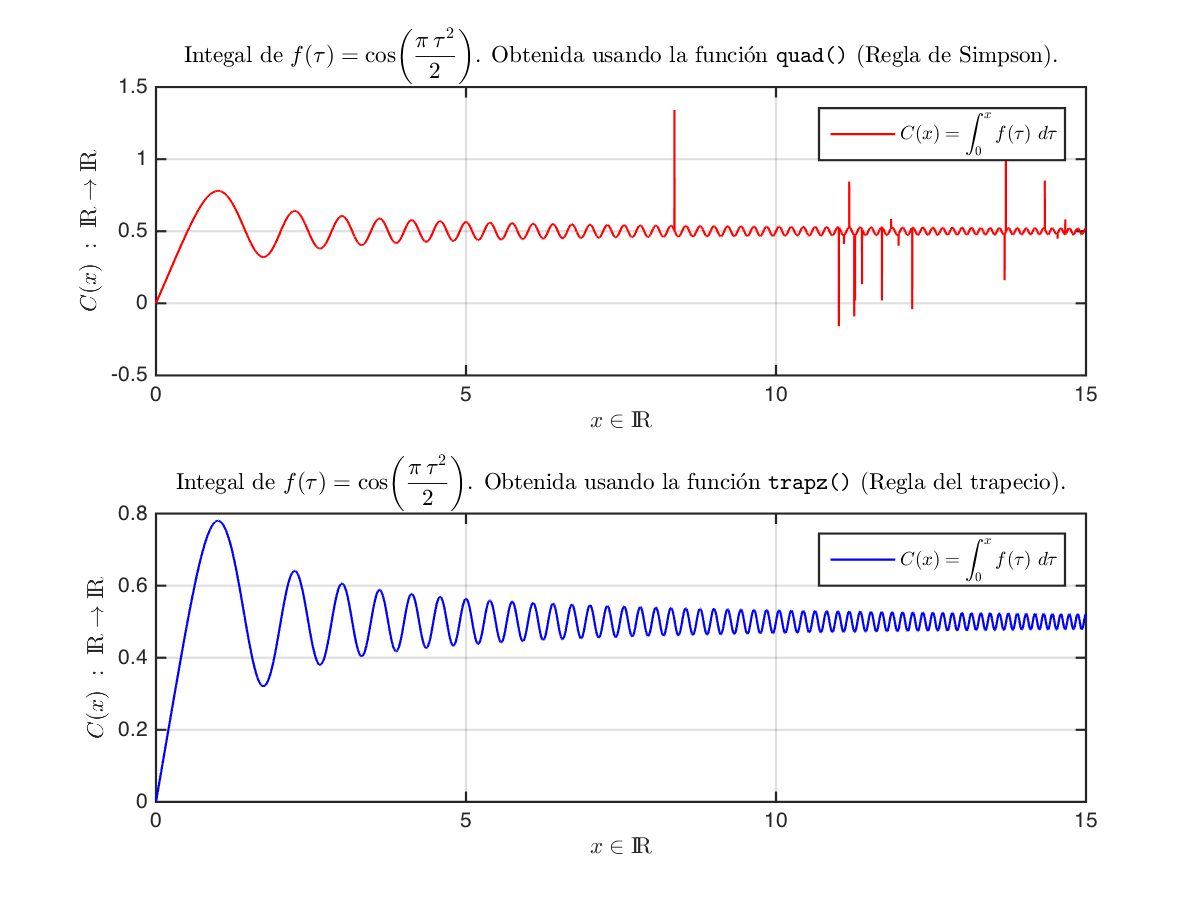
\includegraphics[scale=0.6]{data/img/f1intplot0001}
	\caption{Integral de $f_1(x)$, obtenida numéricamente haciendo uso de las dos funciones referidas, para $0 \leq x \leq 15$, con pasos de 0.001.}
\end{figure}\

\begin{figure}[H]
\centering
	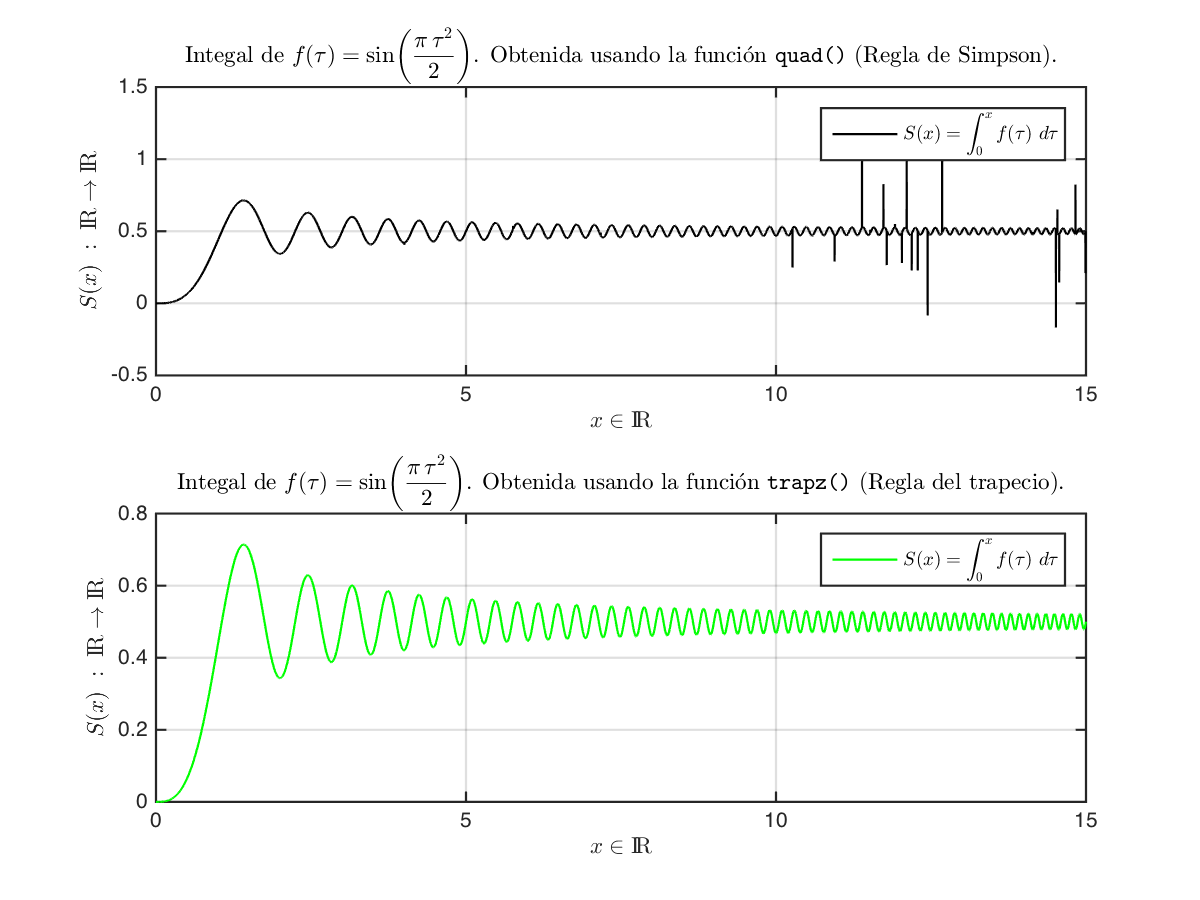
\includegraphics[scale=0.6]{data/img/f2intplot0001}
	\caption{Integral de $f_2(x)$, obtenida numéricamente haciendo uso de las dos funciones referidas, para $0 \leq x \leq 15$, con pasos de 0.001.}
\end{figure}\

\begin{figure}[H]
\centering
	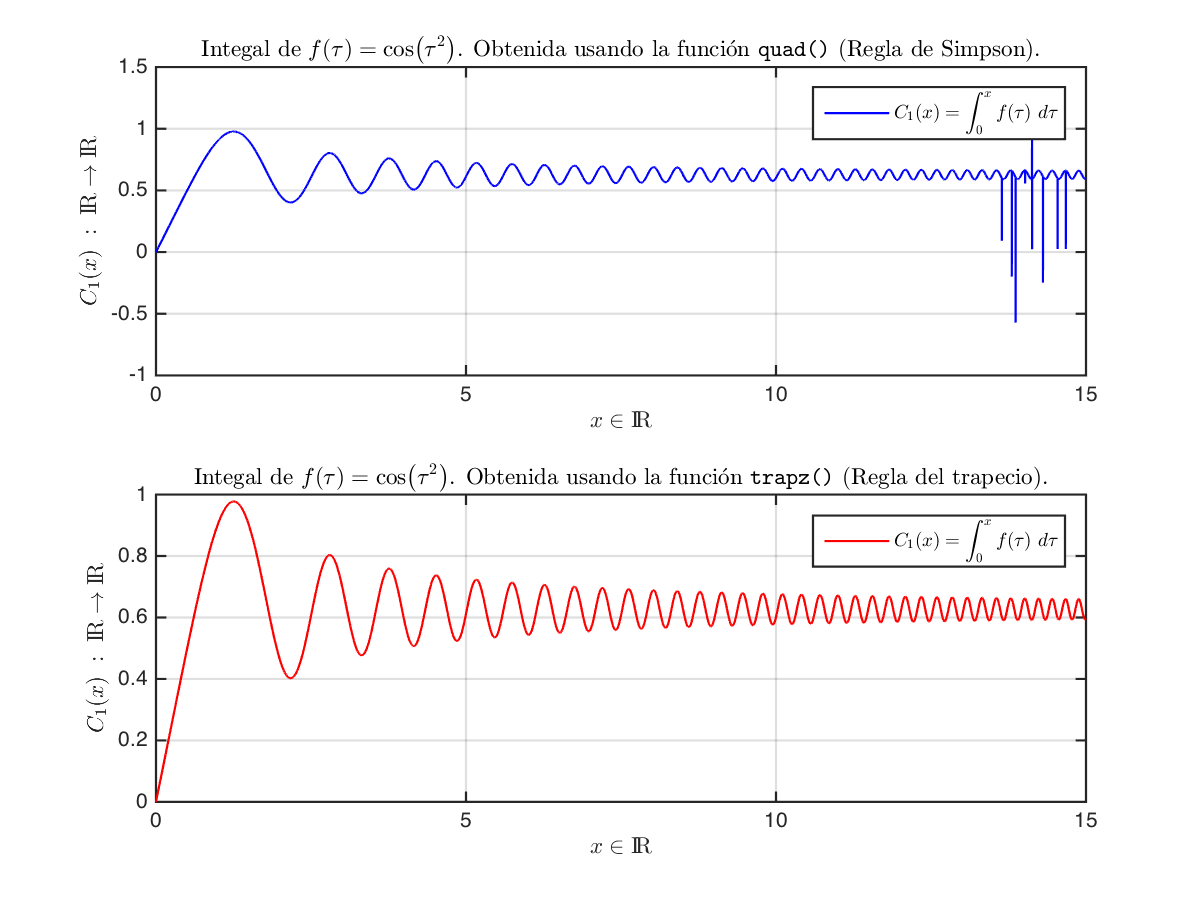
\includegraphics[scale=0.6]{data/img/f3intplot0001}
	\caption{Integral de $f_3(x)$, obtenida numéricamente haciendo uso de las dos funciones referidas, para $0 \leq x \leq 15$, con pasos de 0.001.}
\end{figure}\

\begin{figure}[H]
\centering
	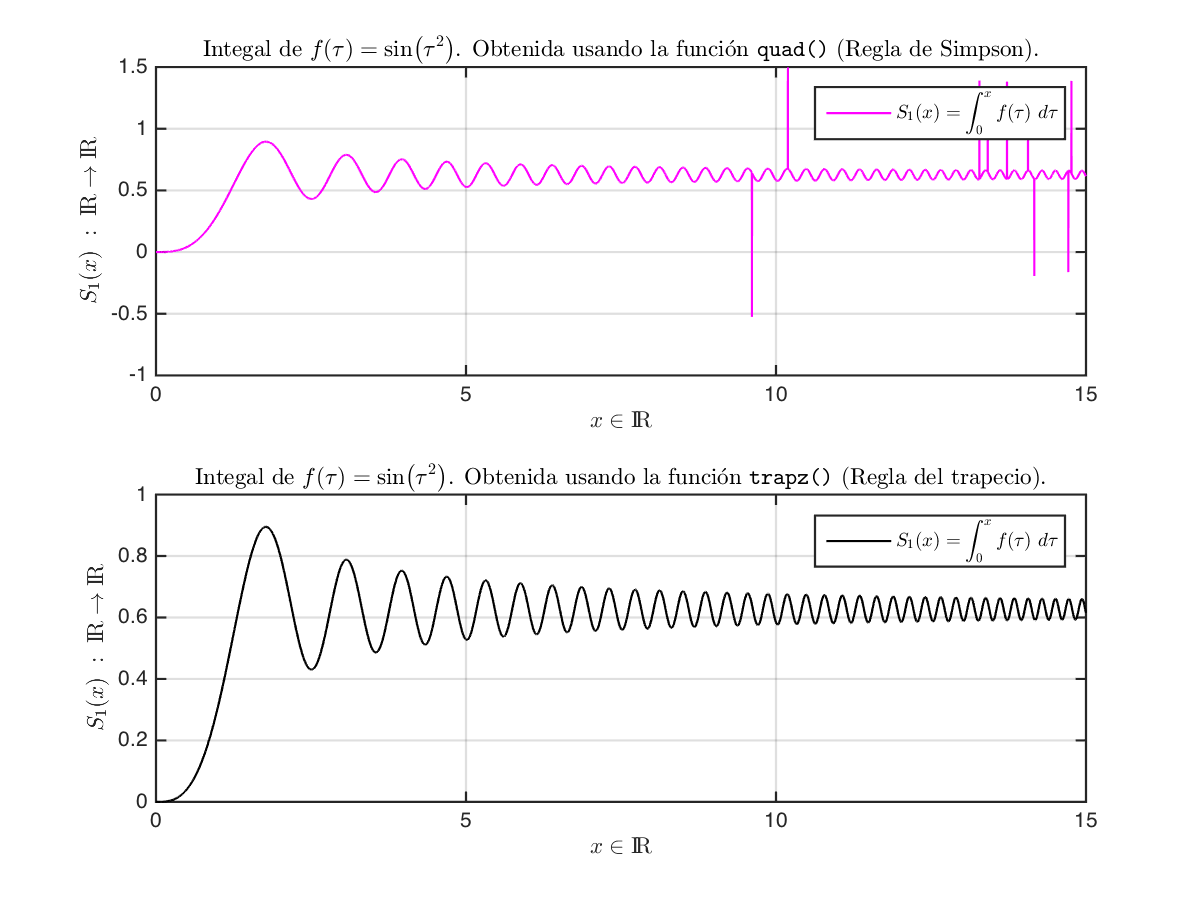
\includegraphics[scale=0.6]{data/img/f4intplot0001}
	\caption{Integral de $f_4(x)$, obtenida numéricamente haciendo uso de las dos funciones referidas, para $0 \leq x \leq 15$, con pasos de 0.001.}
\end{figure}\

\subsection{Método del trapecio y de Simpson en varias dimensiones en \textsc{Matlab}}

Las funciones \texttt{dblquad()}, o \texttt{quad2d()}, y \texttt{triplequad()}, proveen los medios necesarios para calcular la integral iterada, doble o triple de una función en las dimensiones requeridas. A continuación, se incluye la solución de algunas integrales mediante los procedimientos dispuestos por \textsc{Matlab} para esta labor.\\

\begin{itemize}

\item Considérese la siguiente integral:

$$\int_{0}^{1} \int_{0}^{1} \frac{1}{1-xy}\ dy\ dx$$\

Esta integral, puede resolverse en \textsc{Matlab}, haciendo uso de la función \texttt{quad2d}, la cual evalúa de manera numérica una doble integral.\\

La forma general es: \texttt{q = quad2d(fun,a,b,c,d)}, donde se aproxima la funcion \texttt{fun(x, y)}, sobre una región en $\mathbb{R}^2$, $a \leq x \leq x$, y $c(x) \leq y \leq d(x)$. La función, es la función a integrar, y $c$, y $d$, pueden ser valores numéricos. La solución en \textsc{Matlab} de esta integral es a partir de:\\

\lstinputlisting{data/scripts/dintegral1.m}\

El valor de \texttt{i1}, es \texttt{1.6449}.

\item Para la integración triple, es decir la integración iterada en tres dimensiones, la función \texttt{triplequad}, puede ser usada con la forma general \\

\texttt{triplequad(fname,xl,xu,yl,yu,zl,zu)}\\
 
 Donde se tienen el nombre de la función, y los intervalos en cada dimensión. Por ejemplo, la siguiente integral, puede resolverse de la siguiente manera.\
 
$$\int_{0}^{1} \int_{0}^{1} \int_{0}^{1} 64 x y (1-x^2)\ dz\ dy\ dx$$\
 
\lstinputlisting{data/scripts/dintegral2.m}\
 
El valor de \texttt{i2}, es \texttt{1.3333}.

\item Por último, la función \texttt{quad2d}, permite también la integración en el rango de $y$ como funciones de $x$. El siguiente ejemplo ilustra esto:
 
 $$\int_{1}^{2} \int_{x^2}^{x^4} x^2y\ dy\ dx$$\
 
  \lstinputlisting{data/scripts/dintegral3.m}\
  
El valor de \texttt{i3}, es \texttt{83.9740}. La ejemplificación de estos métodos, se encuentra de manera más detallada en las referencias [4] y [7].

\end{itemize}

A partir del desarrollo de los dos últimos scripts, es posible contestar las siguientes preguntas:

\begin{itemize}
\item ¿A qué hacen referencia los parámetros \texttt{AbsTol} y \texttt{RelTol} de las funciones?

Estos parámetros, hacen referencia a la tolerancia absoluta y relativa del método numérico respectivamente, es decir, que tanta tolerancia sobre cada uno de los dos tipos de errores es posible manjar, controlando así, el numero de iteraciones del algoritmo y las presicion de su resultado. El valor por defecto de ellos es $1\times E^5$.

\item ¿Qué métodos usan estos procedimientos?

El método de solución de las integrales triples, resulta de reducir la integral a una doble sobre una función alterada, por lo que es posible entender el desarrollo de las cuadraturas a partir del entendimiento de los métodos que solucionan las integrales dobles en \textsc{Matlab}. El método de solución de las integrales dobles, es a partir de cuadraturas, el cual consiste en aproximar la función dividiendo el plano o el espacio en un grid y calculando el área o el volumen del grid aproximado por la función de integración. El diseño y análisis de estas herramientas de cuadratura, se encuentran en las referencias [1], [2], y [6]. 

\item ¿Qué sucede cuando la función se encuentra indeterminada en algún punto dentro de los límites de integración? ¿Cómo maneja \textsc{Matlab} esta situación?

En este caso, la integral es aproximada mediante la función más cercana a este valor que este definida en este valor.
\end{itemize}

\newpage

%==================================================================
\section{Conclusiones}

El desarrollo de los ejercicios propuestos para el laboratorio, sirvieron para conceptualizar los algoritmos fundamentales para la obtención de la integral de algunas funciones analíticas, definidas como funciones en \textsc{Matlab}, el caso tratado en este laboratorio, es mucho más cercano a cualquier persona por la familiaridad de estas con el cálculo infinitesimal de variables reales. Hallar los valores numéricos de las integrales, resulta muy provechoso para el tratamiento numérico de algunos problemas básicos y algunos avanzados en computación científica.\\

No es suficiente con saber usar las funciones dispuestas en una herramienta de computación científica para el calculo de las integrales, es necesario conocer la pertinencia de cada método, conociendo su funcionamiento interno y los casos de uso. Asimismo, es necesario conocer las ventajas y desventajas de cada uno de los métodos, puede que las desventajas de uno no sea tan perjudicial por la naturaleza del problema a aplicar. Desarrollar herramientas gráficas o estadísticas para visualizar o entender estas diferencias, estas ventajas y desventajas, resulta de gran ayuda en el estudio de los distintos algoritmos numéricos.

%==================================================================

\section{Bibliografía}

\begingroup
\renewcommand{\section}[2]{}%
\begin{thebibliography}{}

\bibitem{lambers1991quad2} Lambers, J. V.  {\em Algorithm QUAD2D: General Two-Dimensional Quadrature.}  1991.

\bibitem{shampine2008266} L.F. Shampine. {\em Matlab program for quadrature in 2D.} 2008. Applied Mathematics and Computation.

\bibitem{yang2005applied} Yang, W.Y. and Cao, W. and Chung, T.S. and Morris, J. {\em Applied Numerical Methods Using MATLAB.} 2005. Wiley. Pags. 50 - 57.

\bibitem{lopez2014matlab} Lopez, C. {\em MATLAB Symbolic Algebra and Calculus Tools.} 2014. MATLAB Solutions Series - Apress. Pags. 73 - 75.

 \bibitem{bradie2006friendly} Bradie, B. {\em A Friendly Introduction to Numerical Analysis.}  2006. Pearson Prentice Hall - Featured Titles for Numerical Analysis Series. Página 150 - 174.
 
 \bibitem{moler2010numerical} Moler, C.B. {\em Numerical Computing with MATLAB: Revised Reprint.} 2010. Society for Industrial and Applied Mathematics. Pags. 65 - 98.

\bibitem{lindfield2012numerical} Lindfield, G. and Penny, J. {\em Numerical Methods: Using MATLAB.} 2012. Elsevier Science. Pags. 281 - 305.

\end{thebibliography}
\endgroup

\bibliography{sample}

\end{document}
